% Make nice A4 pages for print:
%\usepackage{pgfpages}
%\pgfpagesuselayout{resize to}[a4paper,border shrink=5mm,landscape]

\beamertemplatenavigationsymbolsempty

\setbeamertemplate{bibliography item}[text]

\usepackage[type={CC},modifier={by-sa},version={4.0}]{doclicense}

\usepackage[utf8]{inputenc}
\usepackage{hyperref}
\usepackage{breakurl}
\usepackage{graphicx}
\usepackage{pgfplots}
\usepackage{pgf}
\usepackage{tikz}
\usetikzlibrary{positioning}
\usetikzlibrary{arrows}
\usetikzlibrary{decorations.markings}
\usetikzlibrary{calc}
\usetikzlibrary{matrix}
\usetikzlibrary{shapes}
\usetikzlibrary{decorations.pathmorphing}
\usetikzlibrary{fit}
\usetikzlibrary{backgrounds}
\usetikzlibrary{plotmarks}
\usepackage{stmaryrd}
\usepackage{listings}
\usepackage{pdflscape}
\usepackage{perpage}
\usepackage{appendixnumberbeamer}

%\usepackage[thmmarks,amsmath,amsthm]{ntheorem} % already included in beamer
\usepackage{thm-restate}

\usepackage[sort&compress,numbers]{natbib}  % to be have \citet, \citeauthor, \citeyear

\MakePerPage{footnote}

\tikzstyle{o}=[r,ppBlue]
\tikzstyle{r}=[thick,rectangle,align=center]
\tikzstyle{t}=[r,ppTrans] %,font=\bfseries]
\tikzstyle{dd}=[densely dashed]
\tikzstyle{n}=[r,ppBlue]
\tikzstyle{p}=[r,ppRed]
\tikzstyle{ppRed}  =[draw=red,  fill=  red!20]
\tikzstyle{ppBlue} =[draw=blue, fill= blue!20]
\tikzstyle{ppGreen}=[draw=green,fill=green!20]
\tikzstyle{ppTrans}=[draw=none, fill=none]

\usetheme{Warsaw}

\useoutertheme[subsection=true]{smoothbars}
%\useoutertheme[subsection=false]{miniframes}

\definecolor{bblue}{HTML}{D7DF01}	% yellow-ish actually, for better black/white printing
\definecolor{rred}{HTML}{C0504D}
\definecolor{ggreen}{HTML}{9BBB59}
\definecolor{ppurple}{HTML}{9F4C7C}
\definecolor{lightgray}{rgb}{0.3,0.3,0.3}
\definecolor{lightergray}{rgb}{0.9,0.9,0.9}
\definecolor{UniBlue}{RGB}{83,121,170}

\DeclareTextFontCommand\textintro{\normalfont\bfseries\itshape} % nice!
\newcommand{\intro}[2][]
{%
	\textintro{#2}%
}
\newcommand{\empha}[2][]
{%
	\emph{#2}%
}

%\theoremstyle{plain}
\newcounter{reqcounter}
\newtheorem{requirement}[reqcounter]{Requirement}

%setbeamercolor{structure}{fg=violet}

\makeatletter
\def\th@task{%
    \normalfont % body font
    \setbeamercolor{block title example}{bg=orange,fg=white}
    \setbeamercolor{block body example}{bg=orange!20,fg=black}
    \def\inserttheoremblockenv{exampleblock}
  }
\makeatother

\theoremstyle{task}
\newtheorem{task}{Task}

\newenvironment{assignment}%
{%\setbeamercolor{background canvas}{bg=violet}%
%\setbeamercolor{structure}{fg=cyan!90!black}%
 \setbeamercolor{frametitle}{bg=orange,fg=white}
\begin{frame}}%
{\end{frame}}%

\AtBeginSection[]{
  \begin{frame}
  \vfill
  \centering
  \begin{beamercolorbox}[sep=8pt,center,shadow=true,rounded=true]{title}
    \usebeamerfont{title}\insertsectionhead\par%
  \end{beamercolorbox}
  \tableofcontents
  \vfill
  \end{frame}
}




\pgfplotsset{compat=1.14}
\author{Markus Raab}


% TODO: move/split complexity calculations to L10 and/or make clearly optional

\title{L04 Sources of Configuration}

\begin{document}

%%%%%%%%%%%%%%%%%%%%%%%%%%%%%%%%%%%%%%%%%% 
\section{Configuration Files}

% TODO repeat slide
\begin{frame}<1>[label=learning outcomes]
	\frametitle{Learning Outcomes}
	Students will be able to
	\begin{itemize}
	\item differentiate between configuration sources.
	\item unify configuration sources via specifications.
	\item (calculate complexity of configuration settings.)
	\end{itemize}
\end{frame}

\begin{frame}[fragile]
	\frametitle{Definition}
	A \intro{configuration file} is a file containing configuration settings.

	\pause
	A Web server configuration file:

	\begin{lstlisting}[gobble=4]
	port=80 ; comment
	address=127.0.0.1\end{lstlisting}

	\only<2-2>{
	\begin{quest}
	What are keys? What are configuration values? What is metadata?
	\end{quest}
	}
	\pause

	The configuration values are ^80^ and ^127.0.0.1^, respectively.
	Other information in the configuration file is metadata for the configuration settings (such as the comment).
\end{frame}

\begin{frame}
	\frametitle{Configuration File Formats}
	\begin{itemize}
	\item CSV (comma-separated values)
	\item semi-structured
	\item programming language
	\item literate
	\end{itemize}
\end{frame}

\begin{frame}
	\frametitle{CSV formats}
	\begin{itemize}
	\item passwd: \formatdate{3}{11}{1971}
	\item passwd and group use : as separator
	\item are difficult to extend (e.g., GECOS)
	\item today mostly used for legacy reasons
	\item are replaced one-by-one (e.g., inetd, crontab)
	\end{itemize}
\end{frame}

\begin{frame}
	\frametitle{Programming Language}
	\begin{description}
	\item[$+$] trivial for developers (source the file)
	\item[$+$] above-overage quality of error message
	\item[$-$] makes automatic change of individual values harder
	\item[$-$] very hard to use for people who do not know the programming language
	\item[$-$] does not separate code and data
	\end{description}
\end{frame}

\begin{frame}
	\frametitle{Trends}
	\begin{itemize}
	\item away from CSV
	\item towards general-purpose serialization formats (INI, JSON)
	\item human-read/writable (YAML, TOML)
	\item programming language as configuration file
	\end{itemize}
\end{frame}

\begin{frame}
	\frametitle{Method}

	What do FLOSS developers say?

	\begin{description}
	\item[\methodQuestion{}] survey with 672 persons visiting, 162 persons completing the survey~\cite{raab2017challenges}
	\item[\methodSource{}] source code analysis of 16 applications, comprising 50 million lines of code~\cite{raab2017challenges}
	\end{description}
\end{frame}

\begin{frame}
	\frametitle{Why are so many formats present?}
	\methodQuestion{} \question{In which way have you used or contributed to the configuration system/library/API in your previously mentioned FLOSS project(s)?}~\cite{raab2017challenges}
	\begin{itemize}
	\item \p{19} persons ($n=251$) have introduced a configuration file format.
	\item \p{29} implemented a configuration file parser.
	\item \p{15} introduced a configuration system/library/API.
	\item \p{34} used external configuration access APIs.
	\end{itemize}
\end{frame}

\begin{frame}
	\frametitle{Multitude of Formats}
	\begin{itemize}
	\item on every system a multitude of (legacy) configuration file formats exist
	\item the number grows fast
	\item thus applications usually have to deal with some legacy formats
	\end{itemize}
	

	\begin{restatable}{requirement}{reqLegacy}
	A configuration library must be able to integrate (legacy) systems and must fully support (legacy) configuration files.%
	\label{req:legacy}
	\end{restatable}
\end{frame}





%%%%%%%%%%%%%%%%%%%%%%%%%%%%%%%%%%%%%%%%%% 
\section{Command-line Arguments}

\begin{frame}
	\frametitle{Is there something else?}
	\begin{itemize}
	\item configuration files are the most researched of all configuration sources~\cite{jin2014configurations}
	\item but it is neither the most used nor most popular~\cite{raab2017challenges}
	\end{itemize}
\end{frame}

\begin{frame}
	\methodQuestion{} \question{Which configuration systems/libraries/APIs have you already used or would like to use in one of your FLOSS project(s)?}
	\begin{itemize}
	\item command-line arguments (\p{92}, $n=222$)
	\item environment variables (\p{79}, $n=218$)
	\item \methodSource{} API \texttt{getenv} is used omnipresently with 2,683 occurrences
	\item configuration files (\p{74}, $n=218$))
	\end{itemize}
\end{frame}


\begin{frame}
	\methodQuestion{} \question{What is your experience with the following configuration systems/libraries/APIs?}
	\begin{itemize}
	\item \texttt{getenv} (\p{10}, $n=198$)
	\item configuration files (\p{6}, $n=190$)
	\item command-line options (\p{4}, $n=210$)
	\item X/Q/GSettings (\p{41}, \p{14}, \p{35})
	\item KConfig (\p{21})
	\item dconf (\p{42})
	\item plist (\p{32})
	\item Windows Registry (\p{69})
	\end{itemize}
\end{frame}

\begin{frame}<99>[label=semantics command-line arguments]
	\frametitle{Semantics Command-line Arguments}
	\pause
	\begin{itemize}
	\item passed by main for a new process via \\ (\texttt{int argc, char ** argv})
	\item argc might be 0
	\item visible from other processes (e.g., via \texttt{ps aux})
	\item could be passed along to subprocesses but hardly done
	\item need to be parsed by process
	\item portability: differences in parsing
	\item cannot be changed from outside (requires restart, no IPC)
	\end{itemize}
\end{frame}



%%%%%%%%%%%%%%%%%%%%%%%%%%%%%%%%%%%%%%%%%% 
\section{Environment Variables}

\begin{frame}
	\frametitle{Usage}
	\begin{enumerate}
	\item bypassing other configuration accesses (\methodQuestion{} \p{45})
	\item locating configuration files
	\item debugging and testing (\methodQuestion{} \p{55}, \methodSource{} 1,152, i.\,e. \p{43})
	\item sharing configuration settings across applications (\methodQuestion{} \p{53}, \methodSource{} 716, i.\,e. \p{47})
	\item for configuration settings unlikely to be changed by a user (\methodQuestion{} \p{20})
	\item \question{even when it is used inside a loop} (\methodQuestion{} \p{2})
	\end{enumerate}
\end{frame}

\begin{frame}<99>[label=semantics environment variables]
	\frametitle{Semantics Environment Variables}
	\pause
	\begin{itemize}
	\item are also per-process (\texttt{/proc/self/environ})
	\item are not visible from other processes
	\item are automatically inherited by subprocesses
	\item need to be parsed by process (\texttt{[extern] char **environ}) but API is provided (\texttt{getenv})
	\item cannot be changed from outside (requires restart or an additional IPC mechanism)
	\end{itemize}
\end{frame}

\begin{frame}
	\frametitle{getenv}
	\begin{itemize}
	\item is widely standardized, including SVr4, POSIX.1-2001, 4.3BSD, C89, C99~\cite{man2017getenv},
	\item is supported by many programming languages, and
	\item enforces \texttt{key=value} convention.
	\end{itemize}
\end{frame}

\begin{frame}
	\frametitle{Portability}
	\begin{itemize}
	\item no separators for values defined
	\item case sensitivity problems
	\item often many environment variables for the same purpose: TMP, TEMP, or TMPDIR
	\item sometimes one environment variable for different purposes: PATH
	\end{itemize}
\end{frame}





%%%%%%%%%%%%%%%%%%%%%%%%%%%%%%%%%%%%%%%%%% 
\section{Abstractions}

\begin{frame}
	\frametitle{User View}
	\begin{itemize}
	\item command-line for trying out configuration settings
	\item environment variables for configuration settings within a shell
	\item configuration files for persistent configuration settings
	\end{itemize}
\end{frame}

\begin{frame}
	\frametitle{Abstraction}
	\reqLegacy*

	\vspace{1cm}

	How can we deal with the many formats?
\end{frame}

\begin{frame}
	\frametitle{Key-Value}
	A key-value pair is the simplest generic data structure~\cite{strang2004context}.
	While all these formats above have many differences, all of them represent configuration settings as \intro[key-value pair]{key-value pairs}~\cite{jin2014configurations,rabkin2011static,xu2013blame,lathia2013open}.
\\[1cm]

For configuration as program you need to execute them first.
\end{frame}

\begin{frame}
	\frametitle{KeySet (Recapitulation)}

	The common data structure between plugins:
	\vspace{1cm}

	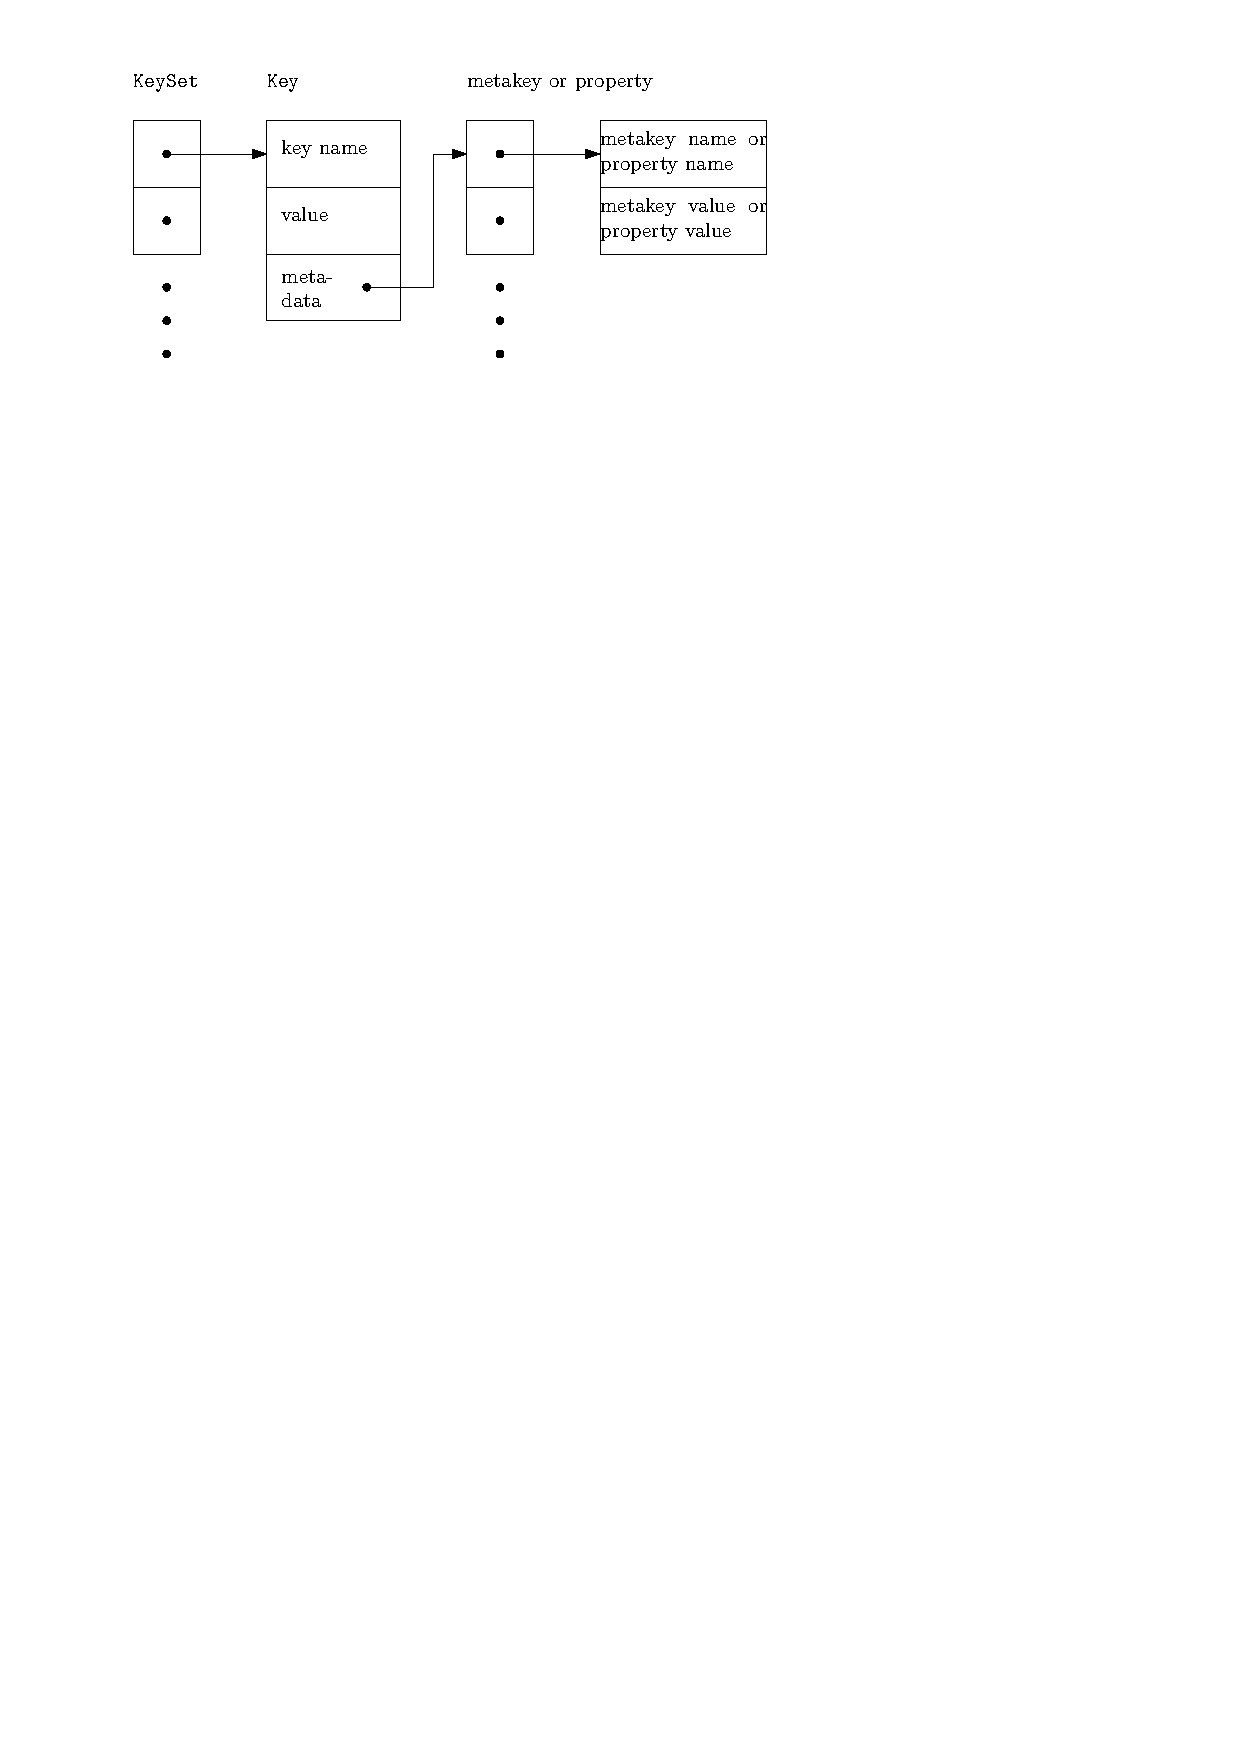
\includegraphics{keyset}
\end{frame}

\begin{frame}
	\frametitle{Mounting}
	\intro[mounting]{Mounting} integrates a backend into the key database~\cite{raab2008thesis}.
	Hence, \elektra{} allows several backends to deal with configuration files at the same time.
	Each backend is responsible for its own subtree of the key database.

	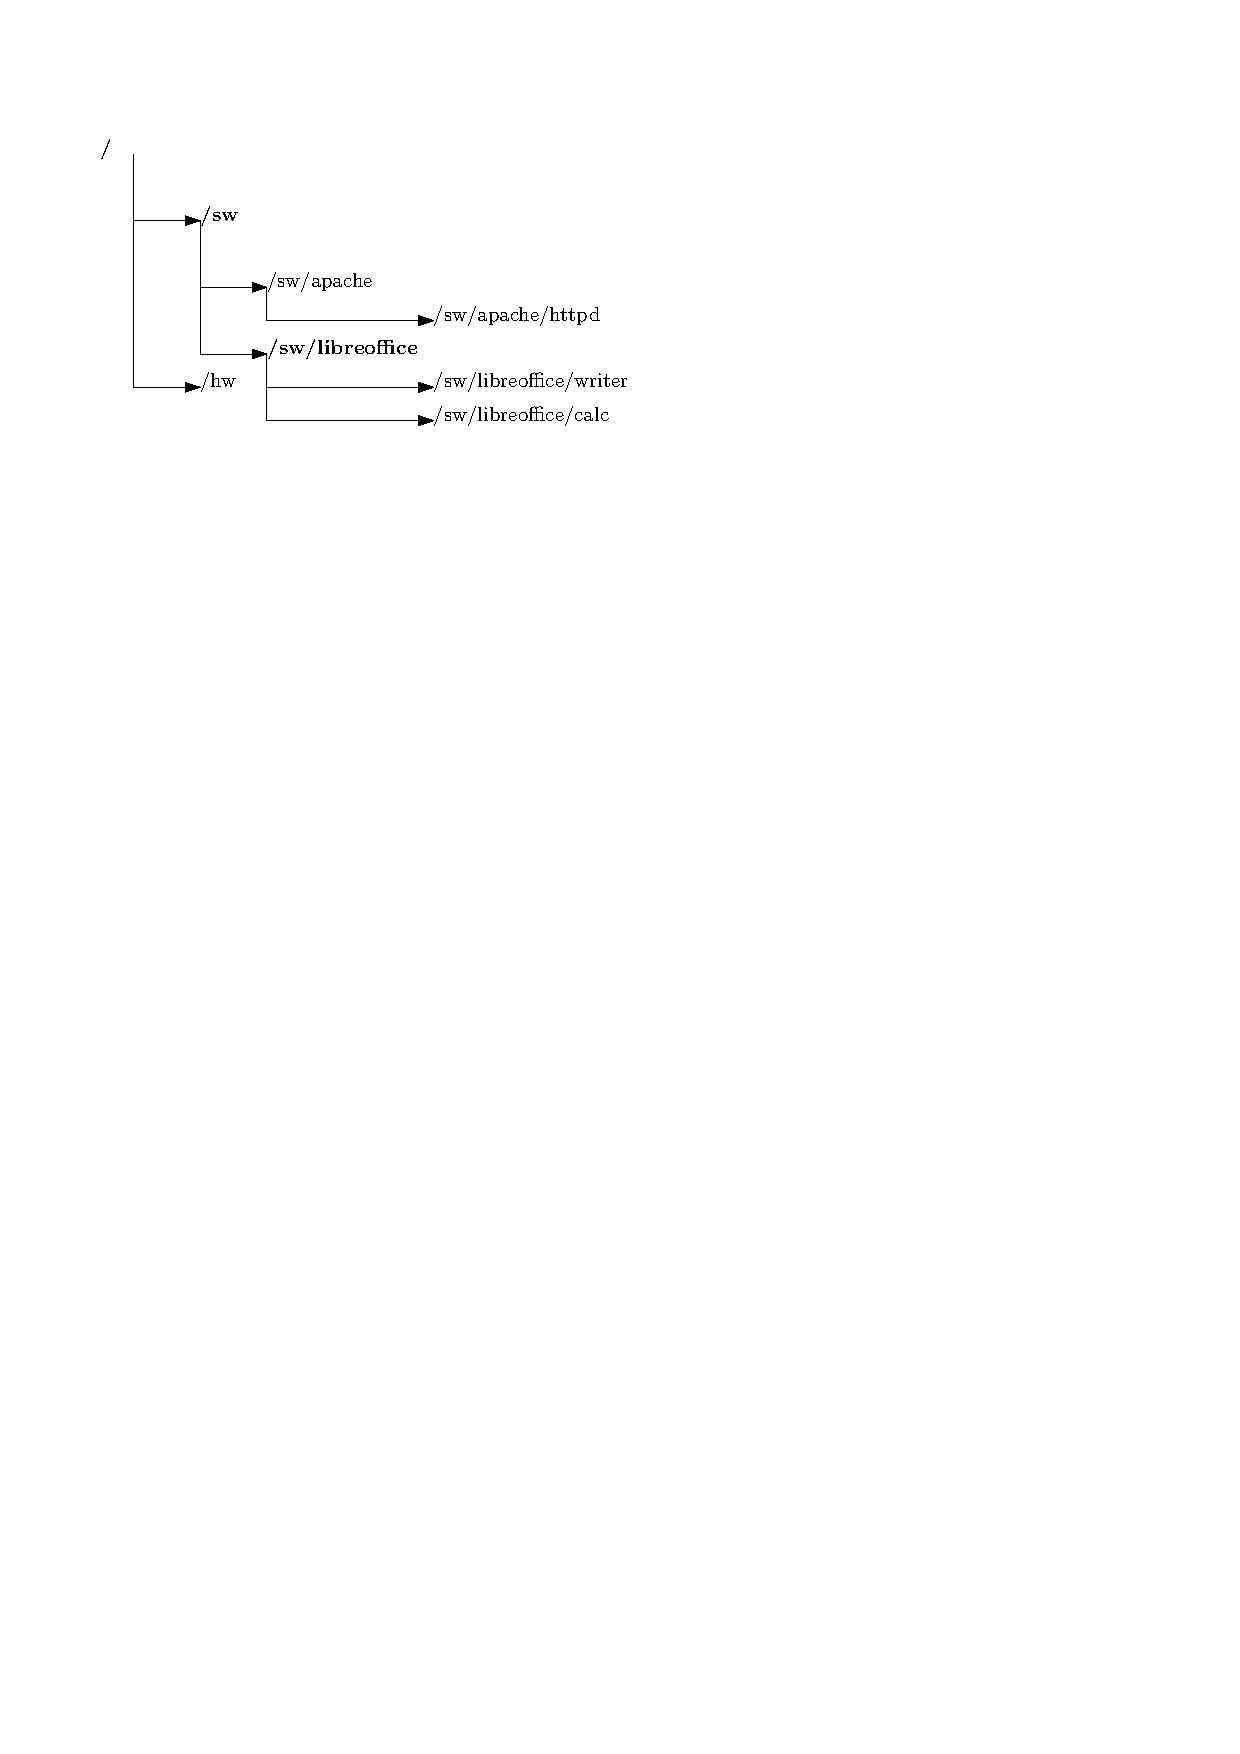
\includegraphics{mounting}
\end{frame}

\begin{frame}[fragile]
	\frametitle{Elektra}

	\begin{code}[gobble=4]
	[kdb/printversion]
	description = "print version information"
	opt = v
	opt/long = version
	opt/arg = none
	\end{code}

	\begin{itemize}
	\item ^gopts^ puts ^Key^s in the ^proc^ namespace
	\item \url{https://www.libelektra.org/tutorials/command-line-options}
	\end{itemize}

	\verb^kdb -v^ \hspace{0.5cm} \verb^kdb --version^ \hspace{0.5cm} \verb^VERSION=1 kdb^
\end{frame}

\begin{frame}
	How can we deal with the many sources?

	\vspace{1cm}

	\begin{restatable}{requirement}{reqEnvironment}
	A configuration library must support all three popular ways for configuration access:
	configuration files, command-line options, and environment variables.
	\end{restatable}
\end{frame}

\begin{frame}
	\frametitle{Plugins}

	Different backends can use different plugins:
	\begin{description}[labelsep=10cm,align=right]
	\item[\texttt{/sw}] in the INI file config.ini
	\item[\texttt{/sw/libreoffice}] in the XML file libreoffice.xml
	\end{description}

	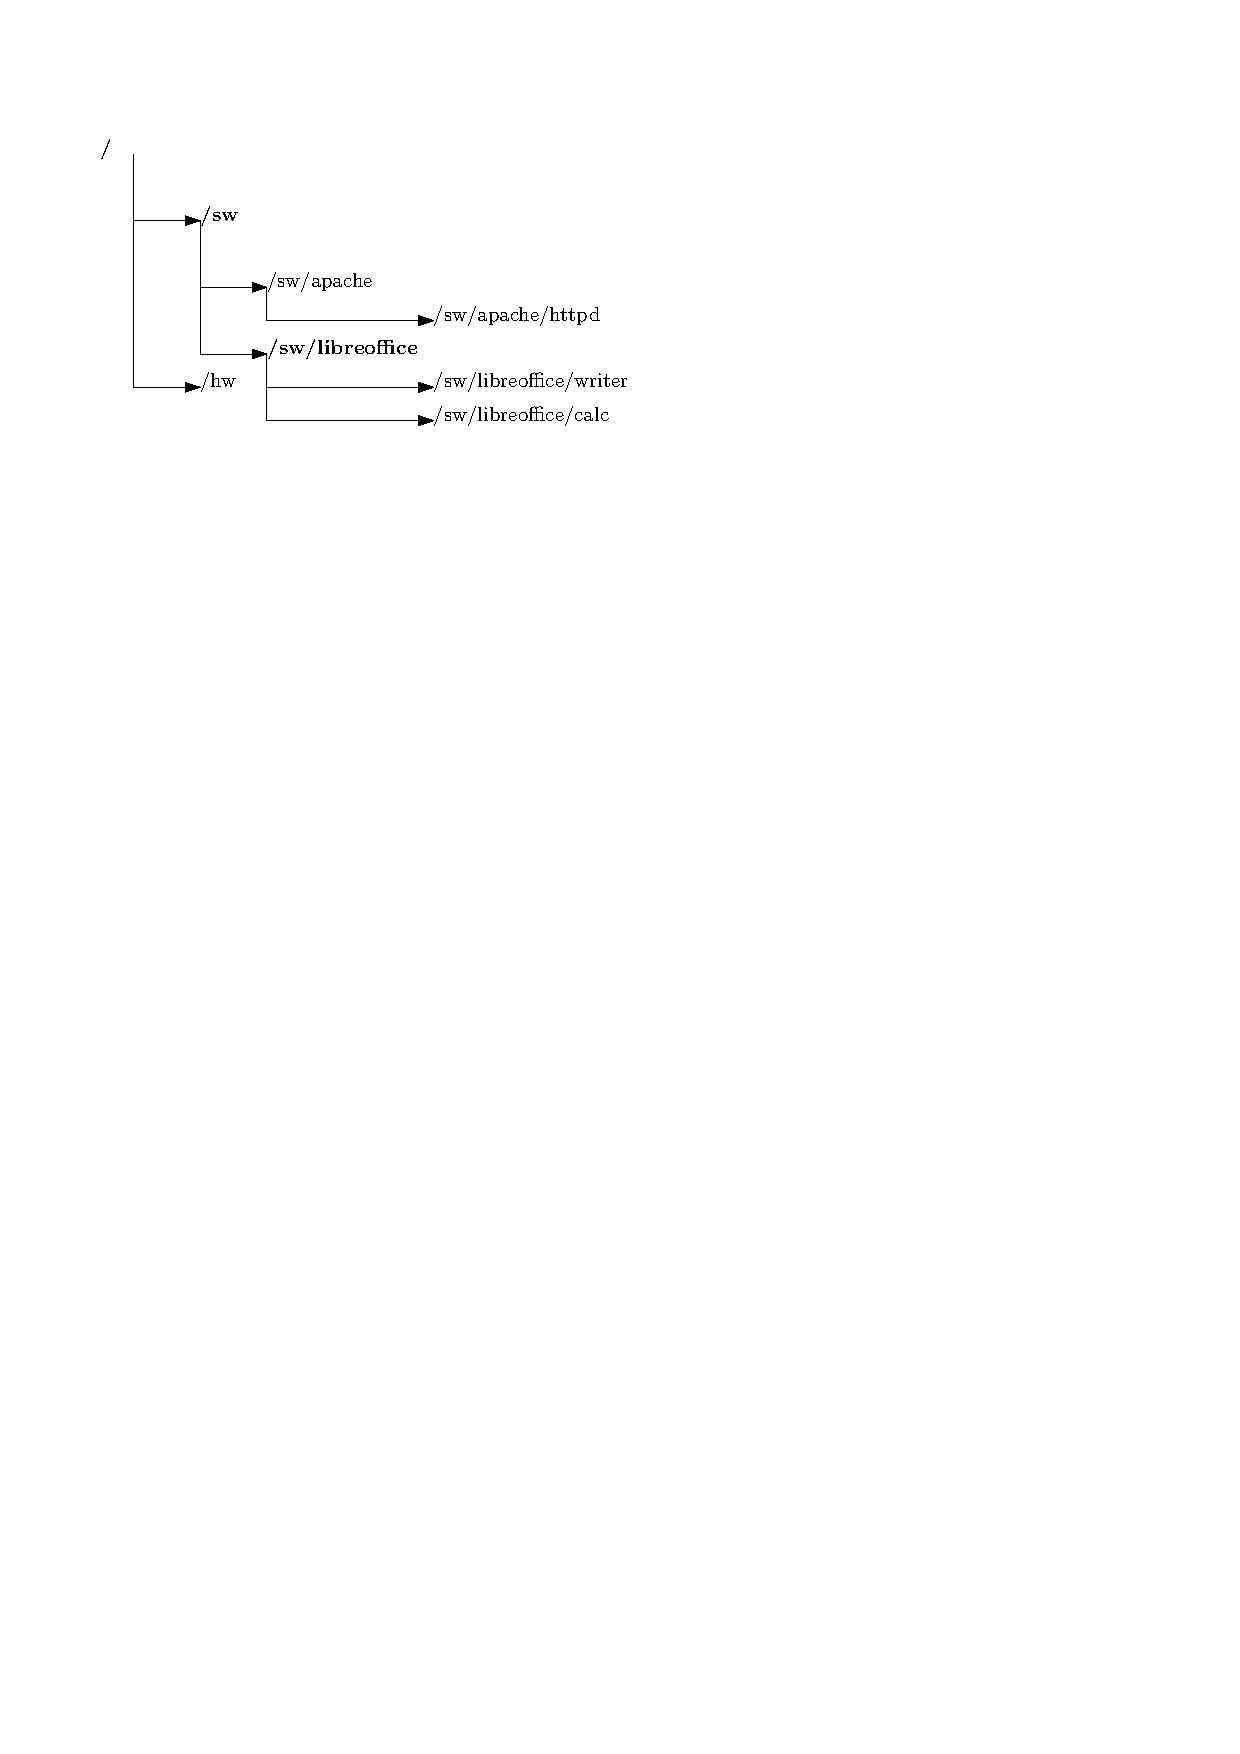
\includegraphics{mounting}
\end{frame}

\begin{frame}
	\frametitle{Cascading}
	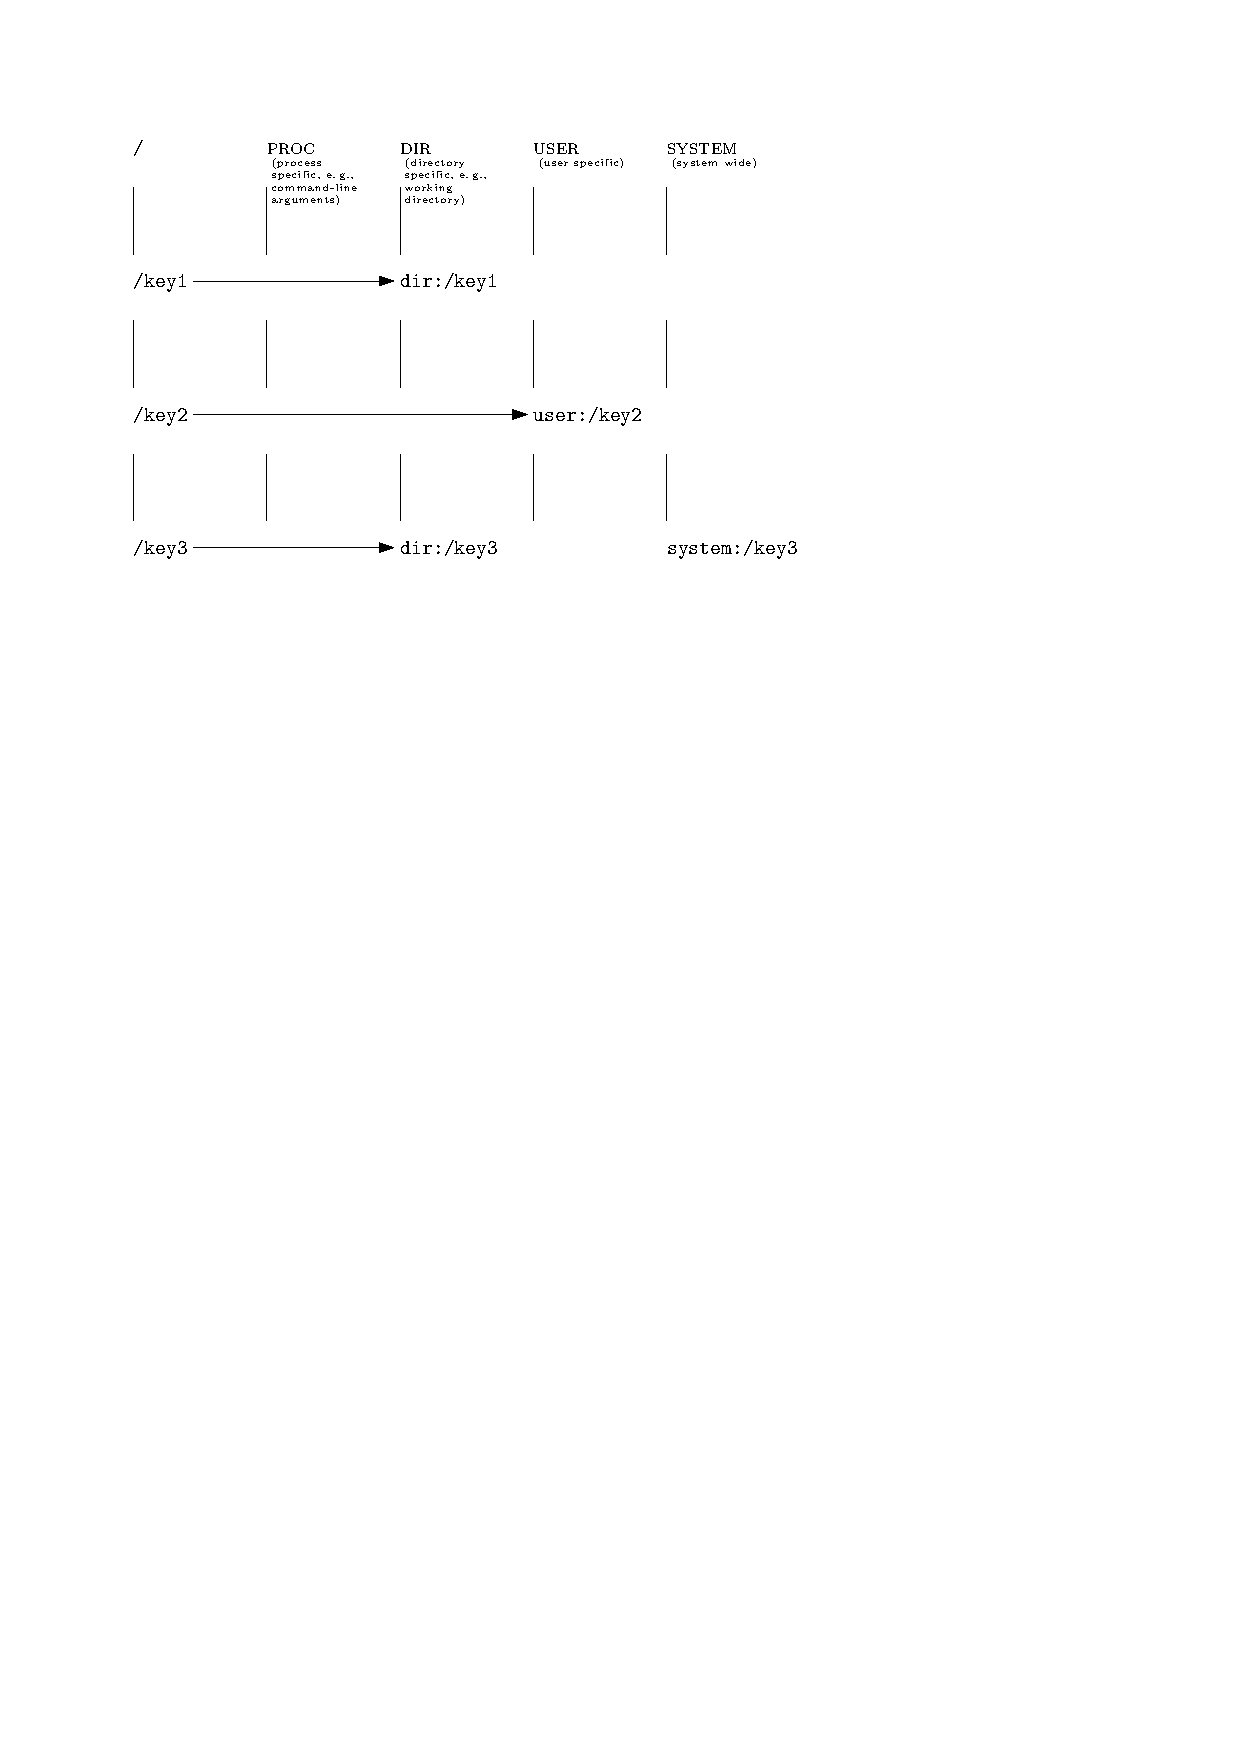
\includegraphics{cascading}
\end{frame}


\begin{frame}
	\frametitle{Conclusion}
	\begin{itemize}
	\item three different configuration sources widely used
	\item all three used for different reasons but often for the same configuration settings
	\item many different configuration file formats
	\item abstractions: key-value, mounting, and cascading
	\end{itemize}
\end{frame}





%%%%%%%%%%%%%%%%%%%%%%%%%%%%%%%%%%%%%%%%%% 
\section{Complexity}

\subsection{Trend}

\begin{frame}
	\frametitle{Trend Firefox}
	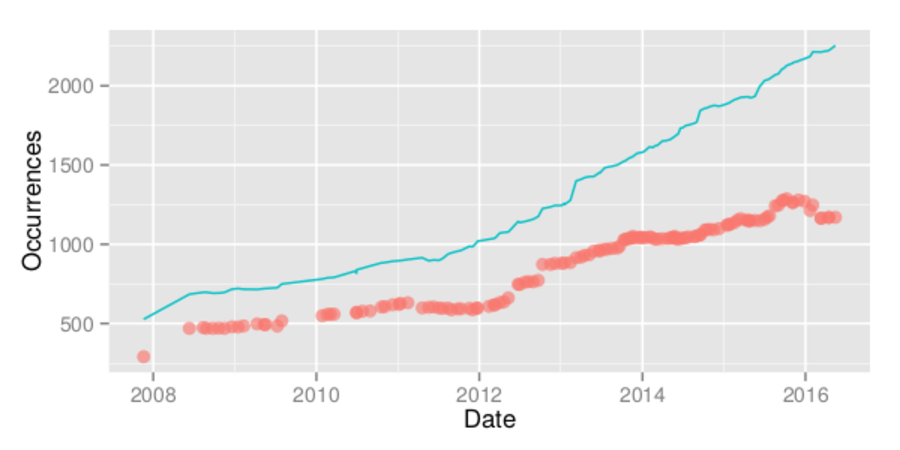
\includegraphics[scale=0.7]{firefox}
\end{frame}

\begin{frame}
	\frametitle{Trend Chromium}
	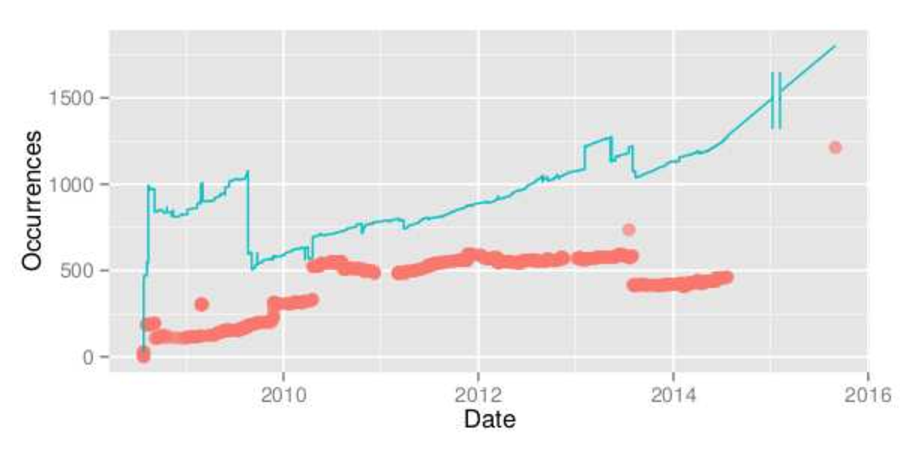
\includegraphics[scale=0.7]{chromium}
\end{frame}

\begin{frame}
	\frametitle{Trend Configuration Files}
	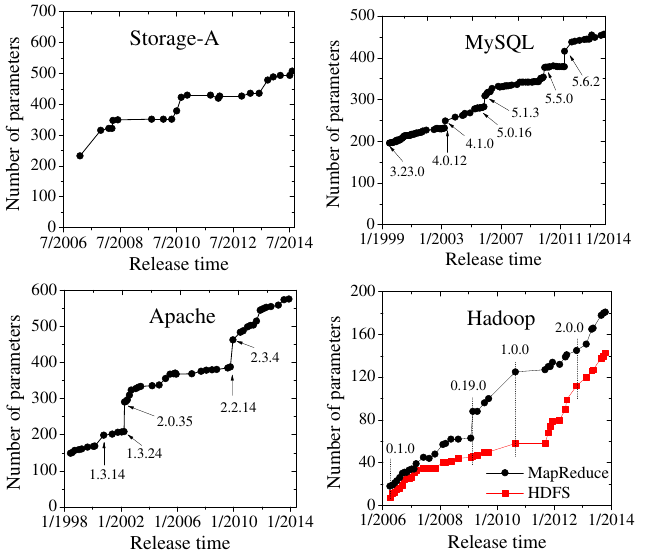
\includegraphics[scale=0.5]{pics/trend.png}
	\citet{xu2015hey}
\end{frame}

\subsection{Calculation}

\begin{frame}
	\frametitle{Types of Complexity}
	\begin{itemize}
	\item complexity in access:
		\begin{itemize}
		\item many different formats
		\item non-uniformity
		\item transformations
		\end{itemize}
	\item configuration settings
		\begin{itemize}
		\item number of settings $s$
		\item number of values $n$
		\item dependences between settings
		\end{itemize}
	\end{itemize}
\end{frame}

\lstDeleteShortInline^
\begin{frame}
	\frametitle{Calculation of Complexity}

	Using enumerative combinatorics:
	\begin{itemize}
	\item number of configurations: $n^s$
	\item for $N$ groups of different $n$ and $s$ (i.e., $n_1 \dots n_N$ with $s_1 \dots s_N$ occurrences):  $$\prod_{i=1}^{N} n_i^{s_i}$$
	\item more difficult to calculate (or unbounded) for dependences, module instantiations, arrays, \dots
	\end{itemize}
\end{frame}

\begin{frame}
	\frametitle{Calculation of Complexity}

	Examples:
	\begin{itemize}
	\item 600 boolean settings in Apache httpd (let us assume $n=2$):
	\pause
	$2^{600} \approx 10^{180}$

	\item 19 integer settings:
	\pause
	${2^{32}}^{19} = 2^{32 \cdot 19} = 2^{609} \approx 10^{183}$

	\item for 20 boolean and 20 enums with 5 possibilities:
	\pause
	$$2^{20}*5^{20} = 10^{20}$$

	\end{itemize}
\end{frame}

\begin{frame}
	\frametitle{Calculation of Complexity (cont.)}

	Examples:
	\begin{itemize}
	\item an array with $1-20$ boolean settings:
	\pause
	$2^{20}$

	\item MySQL has 461 settings, of which 216 are non-simple types~\cite{xu2015hey} \\ (let us assume $n=\{3,20\}$):
	\pause
	$3^{245} * 20^{216} \approx 10^{397}$ \\
	(settings are explained in 5560 pages\footnote{\url{https://downloads.mysql.com/docs/refman-5.7-en.pdf}})
	\end{itemize}
\end{frame}

\begin{frame}
	\frametitle{Calculation of Complexity (cont.)~\cite{jin2014configurations}}

	Examples:
	\begin{itemize}
	\item in Firefox resulting in 846 boolean options and 1,111 options of either integer or string, each with three values

	\pause
	$$2^{846}*3^{1111} \approx 6.46 * 10^{259}$$

	\item LibreOffice
	\pause
	$$2^{4433} * 3^{31889}$$
	\end{itemize}
\end{frame}
\lstMakeShortInline[postbreak=,keywordstyle={},showspaces=no]^
%XXX




%%%%%%%%%%%%%%%%%%%%%%%%%%%%%%%%%%%%%%%%%%
\section{Meeting}

\subsection{Recapitulation}

\againframe<99>{learning outcomes}

\begin{frame}[fragile]
	\frametitle{Definition Configuration File}

	\pause

	A \intro{configuration file} is a file containing configuration settings.

	A Web server configuration file:

	\begin{lstlisting}[gobble=4]
	port=80 ; comment
	address=127.0.0.1\end{lstlisting}

	\only<2-2>{
	\begin{quest}
	What are keys? What are configuration values? What is metadata?
	\end{quest}
	}
	\pause

	The configuration values are ^80^ and ^127.0.0.1^, respectively.
	Other information in the configuration file is metadata for the configuration settings (such as the comment).
\end{frame}

\begin{frame}
	\frametitle{Configuration File Formats}

	\begin{task}
	What are the trends?
	\only<1-1>{
	How can we deal with the many formats?
	}
	\end{task}

	\pause
	\begin{itemize}
	\item away from CSV
	\item towards general-purpose serialization formats (INI, JSON)
	\item human-read/writable (YAML, TOML)
	\item programming language as configuration file
	\end{itemize}

	\only<2-2>{
	\begin{task}
	How can we deal with the many formats?
	\end{task}
	}

	\begin{itemize}
	\item Key-value
	\item Mounting
	\item Plugins
	\end{itemize}
\end{frame}

\begin{assignment}
	\frametitle{Discussion}
	\begin{task}
	What is your favourite configuration file format?
	\end{task}

	\begin{task}
	Did you implement a configuration file parser and/or invented a new configuration file format?
	\end{task}
\end{assignment}

\begin{assignment}
	\begin{task}
	Break.
	\end{task}
\end{assignment}

\begin{assignment}
	\begin{task}
	Optional Reading Text: Handling argc==0 in the kernel.
	\end{task}
\end{assignment}

\againframe<1,2>{semantics command-line arguments}

\againframe<1,2>{semantics environment variables}

\begin{assignment}
	\begin{task}
	What are the differences between mounting and cascading?
	\end{task}
\end{assignment}

\begin{assignment}
	\begin{task}
	Break.
	\end{task}
\end{assignment}

\subsection{Assignments}

\begin{assignment}
	\begin{task}
	CR/LF issue.
	\end{task}
\end{assignment}

\begin{assignment}
	\frametitle{H1 Correction}

	\begin{task}
	Any open questions?
	\end{task}
\end{assignment}

\begin{assignment}
	\frametitle{T0 Correction}

	\begin{task}
	Any missing answers in the issues?
	\end{task}
\end{assignment}

\begin{assignment}
	\frametitle{T1}

	\begin{task}
	Shell Recorder Syntax
	\end{task}
\end{assignment}


\subsection{Preview}

\begin{assignment}
	\begin{task}
	D3: Elektra Plugins
	\end{task}
\end{assignment}


\begin{frame}
	\frametitle{Outlook}

	Will be online during eastern:
	\begin{itemize} %[<+-| alert@+>]
	\item (History of Configuration Management)
	\item CM
	\item CM Tools
	\item Ansible Talk from Lukas Hartl
	\end{itemize}
\end{frame}



\appendix

\begin{frame}[allowframebreaks]
	\bibliographystyle{plainnat}
	\bibliography{../shared/elektra.bib}
\end{frame}


\end{document}
